\documentclass[a4paper,twoside,10pt]{article}
\usepackage[english]{babel}
\usepackage[utf8]{inputenc}
\usepackage{graphicx}
\usepackage{url}
\usepackage[export]{adjustbox}
\usepackage{indentfirst}
% pdflatex

% redefinição das margens das páginas
\setlength{\textheight}{24.00cm}
\setlength{\textwidth}{15.50cm}
\setlength{\topmargin}{0.35cm}
\setlength{\headheight}{0cm}
\setlength{\headsep}{0cm}
\setlength{\oddsidemargin}{0.25cm}
\setlength{\evensidemargin}{0.25cm}

\begin{document}

\begin{figure}[t]
\resizebox{60mm}{!}{
\includegraphics[left]{logoISEL.png}}
\end{figure}

\title{\huge\textbf{Lean Dashboard}}

\author{
\begin{tabular}{l}
José Pedro Jesus, n.º 44805, e-mail: zepedro4259@gmail.com, tel.: 963 730 812\\
Hugo Manuel Jacinto Pinheiro, n.º 44886, e-mail: hugomjp28@gmail.com, tel.: 938 973 719\\
Tomás Simão Mendes dos Santos, n.º 45363, e-mail: tomassms@gmail.com, tel.: 911 029 224\\
\end{tabular}
}

\date{
\begin{tabular}{ll}
  {\textbf{Orientadores:}} & João Pereira, e-mail: joao.pereira@inetum.world, Inetum \\
                 & Filipe Freitas, e-mail: ffreitas@cc.isel.ipl.pt\\
\end{tabular}\\
\vspace{5mm}
\textbf{12 de Abril de 2021}}


\maketitle

\section*{1 - Introduction}
Nowadays, within a company, it is even more important to have an organized and cooperative team with knowledge of all the steps and goals that need to be worked on for the various projects they are currently participating in.
Each member of the team has to keep track of high amounts of information, making it an easy task to overlook or forget issues that might bring problems to a project later on. 

The Lean Dashboard Project will be developed to help the company’s workers keeping track of all the possible tasks for their projects, gathering all the information needed for the various activities such as errors and bugs, test results and staff members from the many sources that are necessary, presenting it on an easy to read and reactive web application. Only certain projects will be available to certain users. To access its projects, a user needs to authenticate. The authentication of users will be managed by a standalone authentication module.

The project will centre around the development of a responsive web application capable of running on a multitude of devices, ranging from smartphones to desktop computers to large screens such as TVs. This web application will display to a work team of a company all of the information regarding various projects being worked on. 
The information being displayed will show the team what needs to be addressed in the project at hands, such as milestones, bugs and current errors in the project.

\pagebreak
\section*{2 - Requirements}
The main problem being addressed with the Lean Dashboard project is the fact that a lot of times, the information relative to a certain work project can be scattered across multiple places, such as different websites, applications and or files.

By putting it all together, we aim to make such info readily available, to not be forgotten and be in plain sight at all times.
As such, the following requirements must be met in order to deliver a functional web application that satisfies the basic needs for the companies.


\section*{2.1 - Database and API}
To manage all of the information, we will first need to develop a back end with NodeJs. Said back end would allow us to retrieve and manage aspects of a project (such as its name or description) as well as its deadlines, bugs and errors. 

The information would be retrieved from various endpoints, adapted to our own and then stored in a PostgreSQL database.

\section*{2.2 - ETL Information Gathering Procedure}
Since the application requires to gather information from a variety of different sources there needs to be implemented an ETL\cite{ETLPROC} (Extract, Transform and Load) procedure so that the API can extract and process the information from the required fonts to later store and present to the user.

\section*{2.3 - User Authentication}
The web application will require a functioning and secure user authentication service.
Such is required so that the information provided to the user will be tailored to the projects they have at hands. The user should only have access to the projects they are currently in a team for.

The developed service will be based on an already existing NodeJS based authentication and authorization component developed as a project for Inetum\cite{INETUM}.

\section*{2.4 - Back Office Management}
The ability to configure the projects and their respective teams.

The back office would be able to manage projects in the application, meaning they would be able to create new projects and update or delete older ones aswell as controling the team members and their functions for said projects. 

They would also have access to a Widget menu that contains data source descriptions and would be able to control the cadence at which the application would access the sources and update the information database including how this information would be presented.

\section*{2.5 - Responsive User Interface}
A responsive and interactive user interface must be implemented so that the application is easy to use and gives them feedback that their action is being/has been processed by the server. The interface will also have to fit various types of screens and devices. The infor can also be displayed in a “Presentation Mode”, in which it will display the various tasks in a slide show, showing the entire team what needs to be addressed in the project development.
It will be developed using a framework such as Angular\cite{ANGULAR}, Webix\cite{WEBIX} or React\cite{REACT}.

\section*{2.6 - Multi Language}
The application’s interface must be developed with multilanguage in mind, as well as the reference data obtained.

\section*{3 - Optional Requirements}
The following requirements would further improve the quality of the project but are planned as Optional.

The focus will be put on the main requirements as they are of most importance to make the application work as intended, however these will be implemented if the project goes smoothly.

\section*{3.1 - Create a BOT}
As an optional requirement, the team would develop a BOT for a communication platform such as slack.
This BOT would be able to interact with the API, retrieve and display data to the user and notify project workers.

\section*{3.2 - Adding Information Sources}
The user would have access to a panel that lets them choose other platforms for the web application to gather information from.

\section*{4 - Techonologies}
The technologies that are planned for the development of this project and their use are the following:
\begin{itemize}
	\item NodeJS will be used to develop the back end.
	\item Front end framework such as Angular\cite{ANGULAR}, Webix\cite{WEBIX} or React\cite{REACT}. The decision of the framework will be made later on as we are still studying each technology in order to decide which one is the most adequate for the project.
	\item Postgres and ElasticSearch. Depending on our data model, we may have to consider only one of these database technologies or both.
\end{itemize}

\section*{5 - System Scheme}

\begin{figure}[!htb]
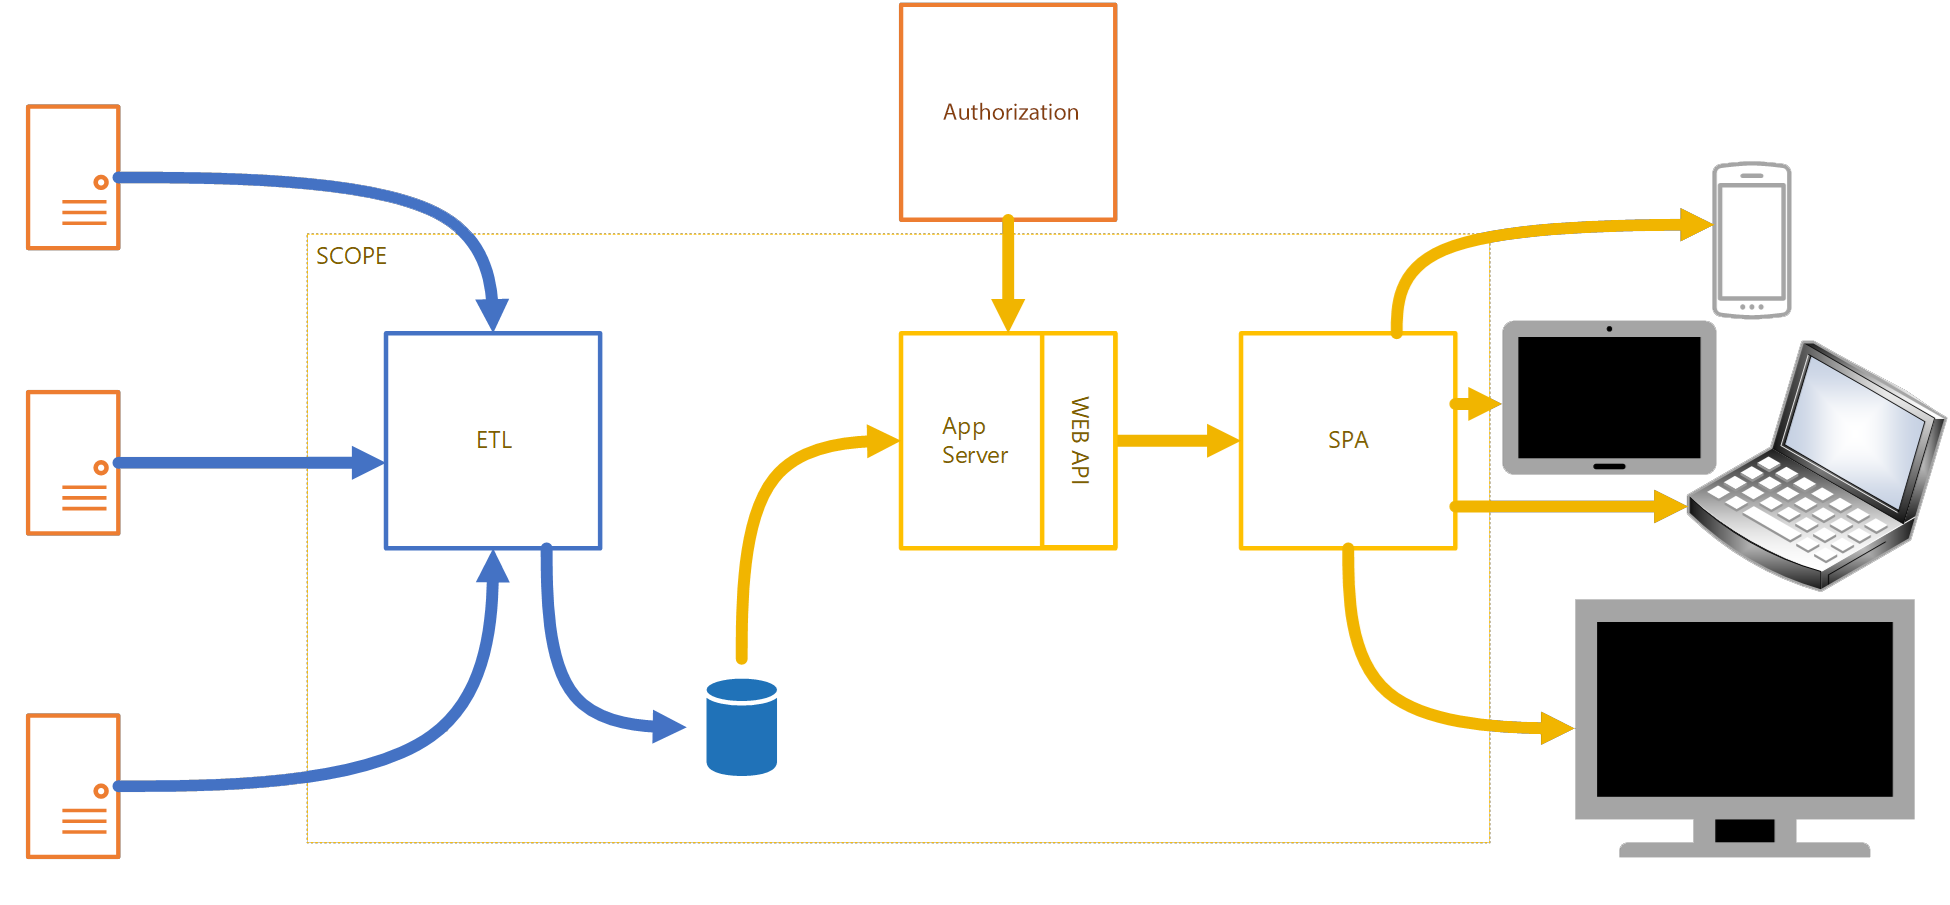
\includegraphics[scale = 0.25, center]{image002.png}
\end{figure}

\pagebreak
\section*{6 - Plan}
\begin{figure}[!htb]

\includegraphics[scale = 0.2, center]{test.png}
\end{figure}

\bibliographystyle{unsrt}
\bibliography{references}

\begin{thebibliography} {websites}
\bibitem{ETLPROC} ETL - Understanding It and Effectively Using It.\\
https://medium.com/hashmapinc/etl-understanding-it-and-effectively-using-it-f827a5b3e54d\\
Consulted on April 1st 2021
\bibitem{INETUM} Inetum\\ https://gfi.world/pt-en/
\bibitem{ANGULAR} Angular\\ https://angular.io
\bibitem{WEBIX} Webix\\ https://webix.com/
\bibitem{REACT} React\\ https://reactjs.org/

\end{thebibliography} 


\end{document}